% ЛИСТОК КРУЖКА 7И, 6.10 — «Раскраски и разрезания». СОБРАН sborka_listka_06-10.py — руками не править.
% Состав финализирован владельцем 05.10 23:08 (Т убрана, две задачи ассистента добавлены 23:35), формат — 05.10 23:23 и 23:27 (SESSIYA.md); проверка: issled/proverka_6-10.py.
\documentclass[11pt,a4paper]{article}
\usepackage{fontspec}
\usepackage{polyglossia}
\setmainlanguage{russian}
\setmainfont{C059}
\usepackage{unicode-math}
\setmathfont{TeX Gyre Schola Math}
\usepackage[left=2.45cm,right=1.3cm,top=1.2cm,bottom=1.0cm]{geometry}
\usepackage{tikz,wrapfig}
\setlength{\parindent}{0pt}
\setlength{\parskip}{13pt plus 3pt}
\linespread{1.07}
\pagestyle{empty}
\newcounter{zad}
\newsavebox{\risbox}
\gdef\wrvverh{0pt}% подъём рисунка над первой строкой задачи (\gdef\wrvverh{…} внутри рисунка)
\gdef\wrlines{}% число строк обтекания вручную (\gdef\wrlines{N} внутри рисунка): wrapfig не считает \parskip и тянет обтекание дальше
% поле для плюсов: ширина 1,25 см; без пунктов — клетка 0,95 см, с пунктами — столбик строк по 0,5 см с буквой
\newcommand{\plusy}[1]{\begin{tikzpicture}[baseline={([yshift=-0.78em]current bounding box.north)}]
  \def\w{1.25}\def\h{0.47}
  \foreach \x [count=\k] in {#1} {\xdef\nk{\k}}
  \ifnum\nk=1
    \draw[line width=0.5pt,rounded corners=1.2pt] (0,0) rectangle (\w,-0.95);
  \else
    \draw[line width=0.5pt,rounded corners=1.2pt] (0,0) rectangle (\w,-\nk*\h);
    \foreach \x [count=\k] in {#1} {
      \node[font=\footnotesize\itshape,anchor=west,inner sep=0pt,text=black!55] at (0.1,{-(\k-0.5)*\h}) {\x};
      \ifnum\k<\nk \draw[line width=0.3pt,black!45] (0,{-\k*\h}) -- (\w,{-\k*\h}); \fi }
  \fi
\end{tikzpicture}}
\newcommand{\ugolok}{
\begin{tikzpicture}[baseline=(current bounding box.south)]
\draw[black!35,line width=0.3pt] (0.000,0.000) rectangle (0.200,-0.200);
\draw[black!35,line width=0.3pt] (0.000,-0.200) rectangle (0.200,-0.400);
\draw[black!35,line width=0.3pt] (0.200,-0.200) rectangle (0.400,-0.400);
\draw[line width=0.9pt,line cap=rect] (0.000,-0.400)--(0.200,-0.400) (0.000,-0.200)--(0.000,-0.400) (0.200,-0.200)--(0.400,-0.200) (0.200,-0.400)--(0.400,-0.400) (0.400,-0.200)--(0.400,-0.400) (0.000,0.000)--(0.200,0.000) (0.000,0.000)--(0.000,-0.200) (0.200,0.000)--(0.200,-0.200);
\end{tikzpicture}}
\newcommand{\tfig}{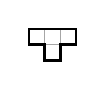
\begin{tikzpicture}[baseline=(current bounding box.south)]
\draw[black!35,line width=0.3pt] (0.000,0.000) rectangle (0.200,-0.200);
\draw[black!35,line width=0.3pt] (0.200,0.000) rectangle (0.400,-0.200);
\draw[black!35,line width=0.3pt] (0.400,0.000) rectangle (0.600,-0.200);
\draw[black!35,line width=0.3pt] (0.200,-0.200) rectangle (0.400,-0.400);
\draw[line width=0.9pt,line cap=rect] (0.200,0.000)--(0.400,0.000) (0.400,0.000)--(0.600,0.000) (0.400,-0.200)--(0.600,-0.200) (0.600,0.000)--(0.600,-0.200) (0.200,-0.400)--(0.400,-0.400) (0.200,-0.200)--(0.200,-0.400) (0.400,-0.200)--(0.400,-0.400) (0.000,0.000)--(0.200,0.000) (0.000,-0.200)--(0.200,-0.200) (0.000,0.000)--(0.000,-0.200);
\end{tikzpicture}}
\newcommand{\zad}[4]{\par\stepcounter{zad}%
  \gdef\wrlines{}\gdef\wrvverh{0pt}\sbox{\risbox}{#4}%
  \ifdim\wd\risbox>0pt
    \ifx\wrlines\empty
      \begin{wrapfigure}{r}{\dimexpr\wd\risbox+14pt\relax}\vspace{\dimexpr-14pt-\wrvverh\relax}\hfill\usebox{\risbox}\vspace{-6pt}\end{wrapfigure}%
    \else
      \begin{wrapfigure}[\wrlines]{r}{\dimexpr\wd\risbox+14pt\relax}\vspace{\dimexpr-14pt-\wrvverh\relax}\hfill\usebox{\risbox}\vspace{-6pt}\end{wrapfigure}%
    \fi
  \fi
  \noindent\llap{\smash{#2}\hspace{0.45cm}}\textbf{\thezad\ifx&#1&\else$^{*}$\fi.}\enspace#3\par}
\newcommand{\shapka}{%
  \noindent{\fontsize{22}{24}\selectfont\bfseries Раскраски и разрезания}\hfill
  {\small Кружок\enspace·\enspace7\,И\enspace·\enspace6 октября}\par
  \vspace{2pt}{\color{black!70}\hrule height 0.6pt}\vspace{10pt}
  \noindent Фамилия, имя\enspace\hrulefill\par\vspace{4pt}
  \setcounter{zad}{0}}

\begin{document}
\shapka

\zad{}{\plusy{а,б}}{Из шахматной доски $8\times8$ вырезали две угловые клетки. Можно ли разрезать оставшуюся часть на доминошки $1\times2$, если вырезали \textbf{(а)}~два угла одной стороны; \textbf{(б)}~два противоположных угла?}{}

\zad{}{\plusy{·}}{Раскрасьте клетки квадрата $4\times4$ в чёрный и белый цвета так, чтобы у каждой чёрной клетки было ровно три белых соседа, а у каждой белой~--- ровно один чёрный сосед (соседи~--- клетки с общей стороной).}{}

\zad{}{\plusy{·}}{Придумайте фигуру из клеток, которую можно вырезать из клетчатой бумаги одним куском и в которой при шахматной раскраске чёрных и белых клеток поровну, но которую нельзя разрезать на доминошки $1\times2$.}{}

\zad{}{\plusy{а,б,в}}{Фишка ходит по доске $5\times5$ на соседнюю по стороне клетку. Можно ли обойти фишкой все клетки, побывав на каждой ровно один раз, если начать \textbf{(а)}~с угловой клетки; \textbf{(б)}~с клетки, соседней с угловой? \textbf{(в)}~С каких клеток можно начать такой обход?}{}

\zad{}{\plusy{а,б}}{Разрежьте по линиям сетки \textbf{(а)}~верхнюю фигуру на три равные части; \textbf{(б)}~нижнюю фигуру на четыре равные части.}{\begin{tabular}{@{}r@{}}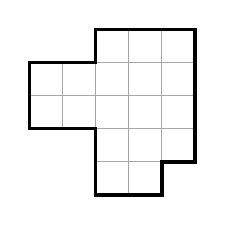
\begin{tikzpicture}[baseline=(current bounding box.north)]
\draw[black!35,line width=0.3pt] (0.840,0.000) rectangle (1.260,-0.420);
\draw[black!35,line width=0.3pt] (1.260,0.000) rectangle (1.680,-0.420);
\draw[black!35,line width=0.3pt] (1.680,0.000) rectangle (2.100,-0.420);
\draw[black!35,line width=0.3pt] (0.000,-0.420) rectangle (0.420,-0.840);
\draw[black!35,line width=0.3pt] (0.420,-0.420) rectangle (0.840,-0.840);
\draw[black!35,line width=0.3pt] (0.840,-0.420) rectangle (1.260,-0.840);
\draw[black!35,line width=0.3pt] (1.260,-0.420) rectangle (1.680,-0.840);
\draw[black!35,line width=0.3pt] (1.680,-0.420) rectangle (2.100,-0.840);
\draw[black!35,line width=0.3pt] (0.000,-0.840) rectangle (0.420,-1.260);
\draw[black!35,line width=0.3pt] (0.420,-0.840) rectangle (0.840,-1.260);
\draw[black!35,line width=0.3pt] (0.840,-0.840) rectangle (1.260,-1.260);
\draw[black!35,line width=0.3pt] (1.260,-0.840) rectangle (1.680,-1.260);
\draw[black!35,line width=0.3pt] (1.680,-0.840) rectangle (2.100,-1.260);
\draw[black!35,line width=0.3pt] (0.840,-1.260) rectangle (1.260,-1.680);
\draw[black!35,line width=0.3pt] (1.260,-1.260) rectangle (1.680,-1.680);
\draw[black!35,line width=0.3pt] (1.680,-1.260) rectangle (2.100,-1.680);
\draw[black!35,line width=0.3pt] (0.840,-1.680) rectangle (1.260,-2.100);
\draw[black!35,line width=0.3pt] (1.260,-1.680) rectangle (1.680,-2.100);
\draw[line width=1.3pt,line cap=rect] (2.100,-0.840)--(2.100,-1.260) (1.680,0.000)--(2.100,0.000) (2.100,0.000)--(2.100,-0.420) (0.420,-1.260)--(0.840,-1.260) (1.680,-1.680)--(2.100,-1.680) (2.100,-1.260)--(2.100,-1.680) (1.260,-2.100)--(1.680,-2.100) (1.680,-1.680)--(1.680,-2.100) (0.420,-0.420)--(0.840,-0.420) (1.260,0.000)--(1.680,0.000) (0.000,-1.260)--(0.420,-1.260) (0.000,-0.840)--(0.000,-1.260) (2.100,-0.420)--(2.100,-0.840) (0.840,-2.100)--(1.260,-2.100) (0.840,-1.680)--(0.840,-2.100) (0.840,0.000)--(1.260,0.000) (0.840,0.000)--(0.840,-0.420) (0.000,-0.420)--(0.420,-0.420) (0.000,-0.420)--(0.000,-0.840) (0.840,-1.260)--(0.840,-1.680);
\end{tikzpicture}\\[10pt]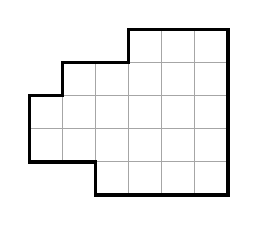
\begin{tikzpicture}[baseline=(current bounding box.north)]
\draw[black!35,line width=0.3pt] (1.260,0.000) rectangle (1.680,-0.420);
\draw[black!35,line width=0.3pt] (1.680,0.000) rectangle (2.100,-0.420);
\draw[black!35,line width=0.3pt] (2.100,0.000) rectangle (2.520,-0.420);
\draw[black!35,line width=0.3pt] (0.420,-0.420) rectangle (0.840,-0.840);
\draw[black!35,line width=0.3pt] (0.840,-0.420) rectangle (1.260,-0.840);
\draw[black!35,line width=0.3pt] (1.260,-0.420) rectangle (1.680,-0.840);
\draw[black!35,line width=0.3pt] (1.680,-0.420) rectangle (2.100,-0.840);
\draw[black!35,line width=0.3pt] (2.100,-0.420) rectangle (2.520,-0.840);
\draw[black!35,line width=0.3pt] (0.000,-0.840) rectangle (0.420,-1.260);
\draw[black!35,line width=0.3pt] (0.420,-0.840) rectangle (0.840,-1.260);
\draw[black!35,line width=0.3pt] (0.840,-0.840) rectangle (1.260,-1.260);
\draw[black!35,line width=0.3pt] (1.260,-0.840) rectangle (1.680,-1.260);
\draw[black!35,line width=0.3pt] (1.680,-0.840) rectangle (2.100,-1.260);
\draw[black!35,line width=0.3pt] (2.100,-0.840) rectangle (2.520,-1.260);
\draw[black!35,line width=0.3pt] (0.000,-1.260) rectangle (0.420,-1.680);
\draw[black!35,line width=0.3pt] (0.420,-1.260) rectangle (0.840,-1.680);
\draw[black!35,line width=0.3pt] (0.840,-1.260) rectangle (1.260,-1.680);
\draw[black!35,line width=0.3pt] (1.260,-1.260) rectangle (1.680,-1.680);
\draw[black!35,line width=0.3pt] (1.680,-1.260) rectangle (2.100,-1.680);
\draw[black!35,line width=0.3pt] (2.100,-1.260) rectangle (2.520,-1.680);
\draw[black!35,line width=0.3pt] (0.840,-1.680) rectangle (1.260,-2.100);
\draw[black!35,line width=0.3pt] (1.260,-1.680) rectangle (1.680,-2.100);
\draw[black!35,line width=0.3pt] (1.680,-1.680) rectangle (2.100,-2.100);
\draw[black!35,line width=0.3pt] (2.100,-1.680) rectangle (2.520,-2.100);
\draw[line width=1.3pt,line cap=rect] (1.260,-2.100)--(1.680,-2.100) (0.420,-1.680)--(0.840,-1.680) (2.100,0.000)--(2.520,0.000) (2.520,0.000)--(2.520,-0.420) (2.520,-0.840)--(2.520,-1.260) (0.840,-2.100)--(1.260,-2.100) (0.840,-1.680)--(0.840,-2.100) (0.000,-1.680)--(0.420,-1.680) (0.000,-1.260)--(0.000,-1.680) (2.100,-2.100)--(2.520,-2.100) (2.520,-1.680)--(2.520,-2.100) (0.840,-0.420)--(1.260,-0.420) (1.680,0.000)--(2.100,0.000) (2.520,-0.420)--(2.520,-0.840) (2.520,-1.260)--(2.520,-1.680) (1.680,-2.100)--(2.100,-2.100) (0.420,-0.420)--(0.840,-0.420) (0.420,-0.420)--(0.420,-0.840) (1.260,0.000)--(1.680,0.000) (1.260,0.000)--(1.260,-0.420) (0.000,-0.840)--(0.420,-0.840) (0.000,-0.840)--(0.000,-1.260);
\end{tikzpicture}\end{tabular}}

\zad{}{\plusy{а,б,в}}{Квадрат $4\times4$ разрезают по линиям сетки на две равные части. Способы, которые получаются друг из друга поворотом или отражением, считаются одинаковыми. \textbf{(а)}~Найдите три разных способа. \textbf{(б)}~Докажите, что линия разреза всегда проходит через центр квадрата. \textbf{(в)}~Найдите все способы.}{}

\zad{}{\plusy{·}}{Разрежьте квадрат $6\times6$ на уголки из трёх клеток\,\ugolok{} так, чтобы никакие два уголка не складывались в прямоугольник $2\times3$.}{}

\zad{}{\plusy{а,б,в}}{\textbf{(а)}~Докажите, что квадрат $3\times3$ нельзя разрезать на уголки из трёх клеток. \textbf{(б)}~Разрежьте на такие уголки квадрат $9\times9$. \textbf{(в)}~При каких $n$ квадрат $n\times n$ можно разрезать на уголки из трёх клеток?}{}

\zad{}{\plusy{·}}{Разрежьте квадрат по линиям сетки на четыре одинаковые части так, чтобы в каждой было по три закрашенные клетки.}{\gdef\wrlines{4}\gdef\wrvverh{20pt}\begin{tabular}{@{}r@{}}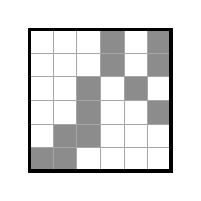
\begin{tikzpicture}[baseline=(current bounding box.north)]
\fill[black!45] (0.900,0.000) rectangle (1.200,-0.300);
\fill[black!45] (1.500,0.000) rectangle (1.800,-0.300);
\fill[black!45] (0.900,-0.300) rectangle (1.200,-0.600);
\fill[black!45] (1.500,-0.300) rectangle (1.800,-0.600);
\fill[black!45] (0.600,-0.600) rectangle (0.900,-0.900);
\fill[black!45] (1.200,-0.600) rectangle (1.500,-0.900);
\fill[black!45] (0.600,-0.900) rectangle (0.900,-1.200);
\fill[black!45] (1.500,-0.900) rectangle (1.800,-1.200);
\fill[black!45] (0.300,-1.200) rectangle (0.600,-1.500);
\fill[black!45] (0.600,-1.200) rectangle (0.900,-1.500);
\fill[black!45] (0.000,-1.500) rectangle (0.300,-1.800);
\fill[black!45] (0.300,-1.500) rectangle (0.600,-1.800);
\draw[black!35,line width=0.3pt] (0.000,0.000) rectangle (0.300,-0.300);
\draw[black!35,line width=0.3pt] (0.300,0.000) rectangle (0.600,-0.300);
\draw[black!35,line width=0.3pt] (0.600,0.000) rectangle (0.900,-0.300);
\draw[black!35,line width=0.3pt] (0.900,0.000) rectangle (1.200,-0.300);
\draw[black!35,line width=0.3pt] (1.200,0.000) rectangle (1.500,-0.300);
\draw[black!35,line width=0.3pt] (1.500,0.000) rectangle (1.800,-0.300);
\draw[black!35,line width=0.3pt] (0.000,-0.300) rectangle (0.300,-0.600);
\draw[black!35,line width=0.3pt] (0.300,-0.300) rectangle (0.600,-0.600);
\draw[black!35,line width=0.3pt] (0.600,-0.300) rectangle (0.900,-0.600);
\draw[black!35,line width=0.3pt] (0.900,-0.300) rectangle (1.200,-0.600);
\draw[black!35,line width=0.3pt] (1.200,-0.300) rectangle (1.500,-0.600);
\draw[black!35,line width=0.3pt] (1.500,-0.300) rectangle (1.800,-0.600);
\draw[black!35,line width=0.3pt] (0.000,-0.600) rectangle (0.300,-0.900);
\draw[black!35,line width=0.3pt] (0.300,-0.600) rectangle (0.600,-0.900);
\draw[black!35,line width=0.3pt] (0.600,-0.600) rectangle (0.900,-0.900);
\draw[black!35,line width=0.3pt] (0.900,-0.600) rectangle (1.200,-0.900);
\draw[black!35,line width=0.3pt] (1.200,-0.600) rectangle (1.500,-0.900);
\draw[black!35,line width=0.3pt] (1.500,-0.600) rectangle (1.800,-0.900);
\draw[black!35,line width=0.3pt] (0.000,-0.900) rectangle (0.300,-1.200);
\draw[black!35,line width=0.3pt] (0.300,-0.900) rectangle (0.600,-1.200);
\draw[black!35,line width=0.3pt] (0.600,-0.900) rectangle (0.900,-1.200);
\draw[black!35,line width=0.3pt] (0.900,-0.900) rectangle (1.200,-1.200);
\draw[black!35,line width=0.3pt] (1.200,-0.900) rectangle (1.500,-1.200);
\draw[black!35,line width=0.3pt] (1.500,-0.900) rectangle (1.800,-1.200);
\draw[black!35,line width=0.3pt] (0.000,-1.200) rectangle (0.300,-1.500);
\draw[black!35,line width=0.3pt] (0.300,-1.200) rectangle (0.600,-1.500);
\draw[black!35,line width=0.3pt] (0.600,-1.200) rectangle (0.900,-1.500);
\draw[black!35,line width=0.3pt] (0.900,-1.200) rectangle (1.200,-1.500);
\draw[black!35,line width=0.3pt] (1.200,-1.200) rectangle (1.500,-1.500);
\draw[black!35,line width=0.3pt] (1.500,-1.200) rectangle (1.800,-1.500);
\draw[black!35,line width=0.3pt] (0.000,-1.500) rectangle (0.300,-1.800);
\draw[black!35,line width=0.3pt] (0.300,-1.500) rectangle (0.600,-1.800);
\draw[black!35,line width=0.3pt] (0.600,-1.500) rectangle (0.900,-1.800);
\draw[black!35,line width=0.3pt] (0.900,-1.500) rectangle (1.200,-1.800);
\draw[black!35,line width=0.3pt] (1.200,-1.500) rectangle (1.500,-1.800);
\draw[black!35,line width=0.3pt] (1.500,-1.500) rectangle (1.800,-1.800);
\draw[line width=1.3pt,line cap=rect] (0.000,-1.200)--(0.000,-1.500) (1.200,-1.800)--(1.500,-1.800) (0.300,-1.800)--(0.600,-1.800) (0.600,0.000)--(0.900,0.000) (1.500,0.000)--(1.800,0.000) (1.800,0.000)--(1.800,-0.300) (0.000,-0.300)--(0.000,-0.600) (1.800,-0.600)--(1.800,-0.900) (0.000,-0.900)--(0.000,-1.200) (1.800,-1.200)--(1.800,-1.500) (0.000,-1.800)--(0.300,-1.800) (0.000,-1.500)--(0.000,-1.800) (0.900,-1.800)--(1.200,-1.800) (0.300,0.000)--(0.600,0.000) (1.200,0.000)--(1.500,0.000) (1.800,-0.300)--(1.800,-0.600) (1.800,-0.900)--(1.800,-1.200) (0.600,-1.800)--(0.900,-1.800) (1.500,-1.800)--(1.800,-1.800) (1.800,-1.500)--(1.800,-1.800) (0.000,0.000)--(0.300,0.000) (0.000,0.000)--(0.000,-0.300) (0.900,0.000)--(1.200,0.000) (0.000,-0.600)--(0.000,-0.900);
\end{tikzpicture}\\[7pt]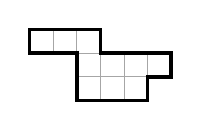
\begin{tikzpicture}[baseline=(current bounding box.north)]
\draw[black!35,line width=0.3pt] (0.000,0.000) rectangle (0.300,-0.300);
\draw[black!35,line width=0.3pt] (0.300,0.000) rectangle (0.600,-0.300);
\draw[black!35,line width=0.3pt] (0.600,0.000) rectangle (0.900,-0.300);
\draw[black!35,line width=0.3pt] (0.600,-0.300) rectangle (0.900,-0.600);
\draw[black!35,line width=0.3pt] (0.900,-0.300) rectangle (1.200,-0.600);
\draw[black!35,line width=0.3pt] (1.200,-0.300) rectangle (1.500,-0.600);
\draw[black!35,line width=0.3pt] (1.500,-0.300) rectangle (1.800,-0.600);
\draw[black!35,line width=0.3pt] (0.600,-0.600) rectangle (0.900,-0.900);
\draw[black!35,line width=0.3pt] (0.900,-0.600) rectangle (1.200,-0.900);
\draw[black!35,line width=0.3pt] (1.200,-0.600) rectangle (1.500,-0.900);
\draw[line width=1.3pt,line cap=rect] (0.300,0.000)--(0.600,0.000) (0.300,-0.300)--(0.600,-0.300) (1.200,-0.900)--(1.500,-0.900) (1.500,-0.600)--(1.500,-0.900) (0.600,-0.300)--(0.600,-0.600) (0.000,0.000)--(0.300,0.000) (0.000,-0.300)--(0.300,-0.300) (0.000,0.000)--(0.000,-0.300) (1.500,-0.300)--(1.800,-0.300) (1.500,-0.600)--(1.800,-0.600) (1.800,-0.300)--(1.800,-0.600) (1.200,-0.300)--(1.500,-0.300) (0.900,-0.900)--(1.200,-0.900) (0.600,0.000)--(0.900,0.000) (0.900,0.000)--(0.900,-0.300) (0.600,-0.900)--(0.900,-0.900) (0.600,-0.600)--(0.600,-0.900) (0.900,-0.300)--(1.200,-0.300);
\end{tikzpicture}\end{tabular}}

\zad{}{\plusy{·}}{Разрежьте фигуру на две равные части. Резать можно не только по сторонам клеток, но и по их диагоналям.}{}

\zad{\star}{\plusy{·}}{Из шахматной доски $8\times8$ вырезали две клетки разного цвета~--- любые. Докажите, что остаток всегда можно разрезать на доминошки.}{}

\zad{\star}{\plusy{а,б}}{Квадрат $8\times8$ разрезали на четыре части, как на рисунке, и сложили из них прямоугольник $5\times13$. \textbf{(а)}~Найдите площадь квадрата и площадь прямоугольника. \textbf{(б)}~Откуда взялась лишняя клетка?}{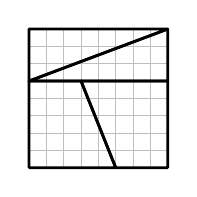
\begin{tikzpicture}[baseline=(current bounding box.north)]
\draw[black!25,line width=0.25pt] (0,0) grid[step=0.22] (1.760,1.760);
\draw[line width=1pt,line join=round] (0.000,1.760)--(1.760,1.760)--(0.000,1.100)--cycle;
\draw[line width=1pt,line join=round] (1.760,1.760)--(1.760,1.100)--(0.000,1.100)--cycle;
\draw[line width=1pt,line join=round] (0.000,0.000)--(1.100,0.000)--(0.660,1.100)--(0.000,1.100)--cycle;
\draw[line width=1pt,line join=round] (1.100,0.000)--(1.760,0.000)--(1.760,1.100)--(0.660,1.100)--cycle;
\end{tikzpicture}\hspace{8pt}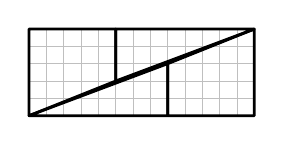
\begin{tikzpicture}[baseline=(current bounding box.north)]
\draw[black!25,line width=0.25pt] (0,0) grid[step=0.22] (2.860,1.100);
\draw[line width=1pt,line join=round] (0.000,0.000)--(1.760,0.000)--(1.760,0.660)--cycle;
\draw[line width=1pt,line join=round] (2.860,1.100)--(1.100,1.100)--(1.100,0.440)--cycle;
\draw[line width=1pt,line join=round] (1.760,0.000)--(2.860,0.000)--(2.860,1.100)--(1.760,0.660)--cycle;
\draw[line width=1pt,line join=round] (0.000,0.000)--(1.100,0.440)--(1.100,1.100)--(0.000,1.100)--cycle;
\end{tikzpicture}}

\end{document}
